\documentclass{article}
\usepackage{amsmath,amssymb,listings,upquote}
\usepackage[margin=3cm]{geometry}
\usepackage{graphicx,color}
\lstset{language=Python}
\usepackage{enumerate}% http://ctan.org/pkg/enumerate
\usepackage{fancyvrb}


\newcounter{zone}
\setcounter{zone}{0}
\newcommand{\zone}{\clearpage\refstepcounter{zone}\section*{Zone \arabic{zone}}}
\newcounter{question}
\setcounter{question}{0}
\newcounter{variant}
\newcounter{questionpoints}
%\newcommand{\question}[1]{\newpage \refstepcounter{question}	
\newcommand{\question}[1]{\refstepcounter{question}
\setcounter{variant}{0} \setcounter{questionpoints}{#1}}
%\newcommand{\variant}{\vspace{4em}\refstepcounter{variant}\noindent \arabic{question}/\arabic{variant}. (\arabic{questionpoints} point\ifnum \thequestionpoints > 1 s\fi) }
\newcommand{\variant}{\vspace{4em}\refstepcounter{variant}\noindent \arabic{question}. (\arabic{questionpoints} point\ifnum \thequestionpoints > 1 s\fi) }
\newenvironment{answers}{\begin{enumerate}}{\end{enumerate}}
\newcommand{\answer}{\item }
%\newcommand{\correctanswer}{\item $\bigstar$ }
\newcommand{\correctanswer}{\item}
\renewcommand{\theenumi}{\Alph{enumi}}
\newenvironment{solution}{{\bf Solution.} }{\vspace*{.3in}\hrule}

\begin{document}

\begin{center}
%\textbf{\Large CS 101 Midterm \#2}
%
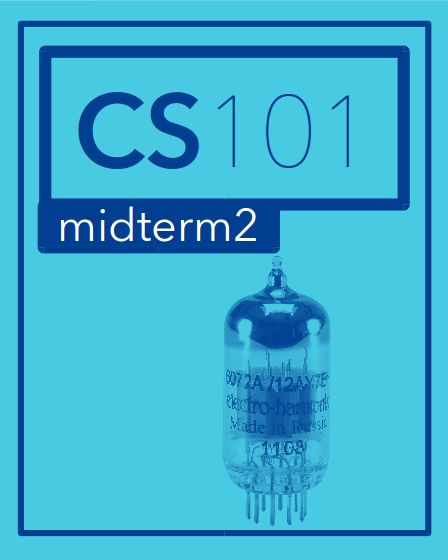
\includegraphics[width=2in]{../img/midterm2-header.png}
\end{center}

\bigskip
\noindent
\begin{itemize}
\item \textbf{Be sure to enter your \underline{full name, student ID} and \underline{your answers to questions} on your answer sheet, being distributed to you separately from this exam booklet}.
\item Do not turn this page until instructed to.
%\item This is a 60-minute exam.
\item There are 30 multiple choice questions worth 1 point each.
\item Each multiple choice question has only \textbf{one} correct answer.
\item You must not communicate with other students during this test.
\item No books, notes, or electronic devices are permitted. In other words, you are not allowed to use a dictionary on your mobile phone or other electronic devices. However, if you don't understand the meaning of a particular English word in this exam, please raise your hand and the instructor will explain the meaning of the English word to you. 
\end{itemize}

\bigskip\bigskip
\noindent
\textbf{\Large Fill in your information:}

\bigskip
{\Large\bf
	\begin{tabular}{ll}
		Full Name: & \underbar{\hskip 8cm} \\[0.5em]
		Student ID: & \underbar{\hskip 8cm} \\[0.5em]
		%NetID: & \underbar{\hskip 8cm}
	\end{tabular}
}

%\bigskip
%\bigskip
%\noindent
%\textbf{\Large 2. Fill in the following answers on the Scantron form:}

%%%%%%%%%%%%%%%%%%%%%%%%%%%%%%%%%%%%%%%%%%%%%%%%%%%%%%%%%%%%%%%%%%%%%%
%%%%%%%%%%%%%%%%%%%%%%%%%%%%%%%%%%%%%%%%%%%%%%%%%%%%%%%%%%%%%%%%%%%%%%
%\zone
\newpage

%%%%%%%%%%%%%%%%%%%%%%%%%%%%%%%%%%%%%%%%%
\question{1}

\variant
Consider the following program:
\begin{Verbatim}
a = 1
def f( a ):
    a = 2 * a
    return a
    a = 3
x = f( a ) + a
\end{Verbatim}
What is the \textbf{value} of \texttt{x} after this program is executed?
\begin{answers}
\answer \texttt{1}
\answer \texttt{2}
\correctanswer \texttt{3}
\answer \texttt{4}
\answer None of the other answers are correct.
\end{answers}
 
 


%%%%%%%%%%%%%%%%%%%%%%%%%%%%%%%%%%%%%%%%%
\question{1}

\variant
Evaluate the following expression:
\begin{Verbatim}
(True or False) or not (False and True)
\end{Verbatim}
What value is produced?
\begin{answers}
\answer \texttt{False}
\correctanswer \texttt{True}
\end{answers}

\vspace{-20pt}
%%%%%%%%%%%%%%%%%%%%%%%%%%%%%%%%%%%%%%%%%
\question{1}

\variant
Consider the following incomplete program.
\begin{Verbatim}
a = "ROBIN"
b = "HOOD "  # note the space
d = { }
for x,y in zip( a,b ):
    ???
s = ""
for c in a:
    s += d[ c ]
print( s )
\end{Verbatim}
What should replace the three question marks to cause this program to print out \texttt{'HOOD '}?
\begin{answers}
\correctanswer \texttt{d[ x ] = y}
\answer \texttt{d[ y ] = x}
\answer \texttt{d[ a ] = b}
\answer \texttt{d[ b ] = a}
\answer \texttt{d[ a ] = x}
\end{answers}
 
 



%%%%%%%%%%%%%%%%%%%%%%%%%%%%%%%%%%%%%%%%%
\question{1}

\variant
Consider the following program.
\begin{Verbatim}
s="".join(["2","0","1"])
x=0
for a,b in enumerate(s):
    x+=a+int(b)
\end{Verbatim}
After it is run, what is the final \textbf{value} of \texttt{x}?
\begin{answers}
\answer \texttt{5}
\answer \texttt{9}
\answer \texttt{3}
\answer \texttt{201}
\correctanswer None of the other answers are correct.
\end{answers}
 
 



%%%%%%%%%%%%%%%%%%%%%%%%%%%%%%%%%%%%%%%%%
\question{1}

\variant
Consider the following program.
\begin{Verbatim}
x='@'
x+='@' # x+='@'
#x+='@'
'''
'''
x+='''@'''
'''
x+='@'
'''
\end{Verbatim}
After it is run, what is the final \textbf{value} of \texttt{x}?
\begin{answers}
\answer \texttt{'@'}
\answer \texttt{'@@'}
\correctanswer \texttt{'@@@'}
\answer \texttt{'@@@@'}
\answer \texttt{'@@@@@'}
\end{answers}
 
 
\newpage

%%%%%%%%%%%%%%%%%%%%%%%%%%%%%%%%%%%%%%%%%
\question{1}

\variant
Consider the following program.
\begin{Verbatim}
d = { }
for a,b in enumerate( '0123456' ):
    d[ b ] = a
x = d[ '2' ] + d[ '1' ]
\end{Verbatim}
After it is run, what is the final \textbf{value} of \texttt{x}?
\begin{answers}
\answer \texttt{1}
\answer \texttt{4}
\answer \texttt{2}
\answer \texttt{5}
\correctanswer \texttt{3}
\end{answers}
 
 

%%%%%%%%%%%%%%%%%%%%%%%%%%%%%%%%%%%%%%%%%
\question{1}
\variant
Evaluate the following expression:
\begin{Verbatim}
len(",3,4,5,6,7,".split(','))
\end{Verbatim}
\begin{answers}
\answer \texttt{5}
\answer \texttt{6}
\correctanswer \texttt{7}
\answer \texttt{25}
\answer \texttt{'34567'}
\end{answers}
 
 
 

%%%%%%%%%%%%%%%%%%%%%%%%%%%%%%%%%%%%%%%%%
\question{1}
\variant
Consider the following program.
\begin{Verbatim}
a,b = "KING","JOHN"
def f( a,b ):
    return b,a
x = ','.join( f( a,b ) )
\end{Verbatim}
After it is run, what is the final \textbf{value} of \texttt{x}?
\begin{answers}
\answer \texttt{"KING","JOHN"}
\answer \texttt{"JOHN","KING"}
\answer \texttt{"KING,JOHN"}
\correctanswer \texttt{"JOHN,KING"}
\answer None of the other answers are correct
\end{answers}
 

%%%%%%%%%%%%%%%%%%%%%%%%%%%%%%%%%%%%%%%%%
\question{1}

\variant
Consider the following program.
\begin{Verbatim}
a,b = "MAID","MARIAN"
def f( a,b ):
    return "%sx%d" % (a , len(b))
    b,a = a,b
x = f( a,b )
\end{Verbatim}
After it is run, what is the final \textbf{value} of \texttt{x}?
\begin{answers}
\answer \texttt{"MAID",6}
\answer \texttt{"MARIAN",4}
\answer \texttt{"MAIDxMARIAN"}
\correctanswer \texttt{"MAIDx6"}
\answer None of the other answers are correct
\end{answers}
 
 

%%%%%%%%%%%%%%%%%%%%%%%%%%%%%%%%%%%%%%%%%
\question{1}

\variant
Consider the following program.
\begin{Verbatim}
import numpy as np
x=np.array([ [1,2] ]*2)+1
\end{Verbatim}
After it is run, what is the final \textbf{value} of \texttt{x}?
\begin{answers}
\correctanswer $ \left[ \begin{array}{cc} 2 & 3 \\ 2 & 3 \\ \end{array} \right] $
\answer $ \left[ \begin{array}{cc} 3 & 5 \\ \end{array} \right] $
\answer $ \left[ \begin{array}{c} 3 \\ 5 \\ \end{array} \right] $
\answer $ \left[ \begin{array}{cccc} 2 & 3 & 2 & 3 \\ \end{array} \right] $
\answer None of the other answers are correct
\end{answers}
 
 
\newpage

%%%%%%%%%%%%%%%%%%%%%%%%%%%%%%%%%%%%%%%%%
\question{1}

\variant
Consider the following 2-dimensional numpy array:
$$
\left[ \begin{array}{ccc} 1 & 2 & 3 \\ 4 & 5 & 6 \\ 7 & 8 & 9 \\ 10 & 11 & 12 \\ \end{array} \right]
$$
Assuming it is stored in a variable named \texttt{a}, how can we index and retrieve the value 6?
\begin{answers}
\correctanswer \texttt{a[1][2]}
\answer \texttt{a[2][1]}
\answer \texttt{a[2][3]}
\answer \texttt{a[3][2]}
\end{answers}
 
 


%%%%%%%%%%%%%%%%%%%%%%%%%%%%%%%%%%%%%%%%%
\question{1}

\variant
Consider the following 2-dimensional array:
$$
\left[ \begin{array}{ccc} 6 & 5 & 4 \\ 3 & 2 & 1 \\ \end{array} \right]
$$
Which of the following expressions will generate this array?
\begin{answers}
\correctanswer \texttt{np.array([ [6,5,4], [3,2,1] ])}
\answer \texttt{np.array([ [6,3], [5,2], [4,1] ])}
\answer \texttt{np.array([ [6,5], [4,3], [2,1] ])}
\answer \texttt{np.array([ [6,5,4,3,2,1] ])}
\end{answers}
 
 


%%%%%%%%%%%%%%%%%%%%%%%%%%%%%%%%%%%%%%%%%
\question{1}

\variant
Consider the following program.
\begin{Verbatim}
d = { "T":2,"U":1,"C":4,"K":1 }
for c in "FRIAR":
    print( d[ c ] + 3 )
\end{Verbatim}
What kind of exception will this program throw?
\begin{answers}
\correctanswer \texttt{KeyError: 'F'}
\answer \texttt{TypeError: list indices must be integers, not str}
\answer \texttt{SyntaxError: invalid syntax}
\answer \texttt{TypeError: unsupported operand type(s) for +: 'str' and 'int'}
\end{answers}
 
 
 \newpage

%%%%%%%%%%%%%%%%%%%%%%%%%%%%%%%%%%%%%%%%%
\question{1}

\variant
Consider the following program.
\begin{Verbatim}
import numpy as np
x = np.zeros( ( 3,3 ) )
for i in range( 3 ):
    for j in range( 3 ):
        x[ i ][ j ] = i*i + j
\end{Verbatim}
After it is run, what is the final \textbf{value} of \texttt{x}?
\begin{answers}
\answer $ \left[ \begin{array}{ccc} 0 & 1 & 4 \\ 1 & 2 & 5 \\ 2 & 3 & 6 \end{array} \right] $
\correctanswer $ \left[ \begin{array}{ccc} 0 & 1 & 2 \\ 1 & 2 & 3 \\ 4 & 5 & 6 \end{array} \right] $
\answer $ \left[ \begin{array}{ccc} 0 & 1 & 2 \\ 0 & 2 & 4 \\ 0 & 3 & 6 \end{array} \right] $
\answer $ \left[ \begin{array}{ccc} 0 & 0 & 0 \\ 1 & 2 & 3 \\ 2 & 4 & 6 \end{array} \right] $
\answer None of the other answers are correct
\end{answers}
 
 
  \newpage

%%%%%%%%%%%%%%%%%%%%%%%%%%%%%%%%%%%%%%%%%
\question{1}

\variant
Consider the following program.
\begin{Verbatim}
import numpy as np
x = np.zeros( ( 3,3 ) )
for i in range( 3 ):
    x[ i,i ] = 1
    for j in range( 3 ):
        if i < j:
            continue
        x[ i,j ] = 2
\end{Verbatim}
After it is run, what is the final \textbf{value} of \texttt{x}?
\begin{answers}
\correctanswer $ \left[ \begin{array}{ccc} 2 & 0 & 0 \\ 2 & 2 & 0 \\ 2 & 2 & 2 \end{array} \right] $
\answer $ \left[ \begin{array}{ccc} 1 & 2 & 2 \\ 2 & 1 & 2 \\ 2 & 2 & 1 \end{array} \right] $
\answer $ \left[ \begin{array}{ccc} 1 & 0 & 0 \\ 2 & 1 & 0 \\ 2 & 2 & 1 \end{array} \right] $
\answer $ \left[ \begin{array}{ccc} 1 & 2 & 2 \\ 0 & 1 & 2 \\ 0 & 0 & 1 \end{array} \right] $
\answer $ \left[ \begin{array}{ccc}  2 & 2 & 2 \\ 0 & 2 & 2 \\ 0 & 0 & 2 \end{array} \right] $
\end{answers}
 
 

%%%%%%%%%%%%%%%%%%%%%%%%%%%%%%%%%%%%%%%%%
\question{1}
\variant
Consider the following program.
\begin{Verbatim}
a = [ "1",2,"3",0 ]
x = 0
for e in a:
    try:
        x += e
    except:
        x += 1
\end{Verbatim}
After it is run, what is the final \textbf{value} of \texttt{x}?
\begin{answers}
\answer \texttt{1}
\answer \texttt{2}
\answer \texttt{3}
\correctanswer \texttt{4}
\answer \texttt{5}
\end{answers}
 
 

 

%%%%%%%%%%%%%%%%%%%%%%%%%%%%%%%%%%%%%%%%%
\question{1}

\variant
Consider the following program.
\begin{Verbatim}
x = "1 2 3".split()
x = ','.join( x )
try:
    print( x.append( 4 ) )
except:
    print( type( x ) )
\end{Verbatim}
After it is run, what is printed by this program?
\begin{answers}
\answer \texttt{TypeError}
\answer \texttt{[ 1,2,3,4 ]}
\answer \texttt{<class 'list'>} (output from calling the \texttt{type} function on a list)
\correctanswer \texttt{<class 'str'>} (output from calling the \texttt{type} function on a string)
\end{answers}
 
 

%%%%%%%%%%%%%%%%%%%%%%%%%%%%%%%%%%%%%%%%%
\question{1}
\variant
Consider the following incomplete program:
\begin{Verbatim}
x = "TUCK"
y = "CKTU"
z = ""
???
print( z )
\end{Verbatim}
Replacing the three question marks with which of the following will result in an output of \texttt{"TUCK"}?
\begin{answers}
\correctanswer
\begin{Verbatim}
for a in x:
    for b in y:
        if a == b:
            z += b
\end{Verbatim}
\answer
\begin{Verbatim}
for a in y:
    for b in x:
        if a == b:
            z += b
\end{Verbatim}
\answer
\begin{Verbatim}
for a in x:
    for b in y:
        if a != b:
            z += b
\end{Verbatim}
\answer
\begin{Verbatim}
for a in y:
    for b in x:
        if a != b:
            z += b
\end{Verbatim}
\end{answers}
 
 
\newpage

%%%%%%%%%%%%%%%%%%%%%%%%%%%%%%%%%%%%%%%%%%%%%
\question{1}

\variant
For this problem, your job is to put the lines of code below in the proper order to create a function that accomplishes a task. We will completely ignore indentation.
\begin{enumerate}[1]
\item  \texttt{except:}
\item  \texttt{def is\_close( a,b,rtol=1e-3 ):}
\item  \texttt{try:}
\item  \texttt{return None}
\item  \texttt{def is\_close( a,b,rtol )}
\item  \texttt{rtol = 1e-3}
\item  \texttt{return ( abs(a-b)/abs(b) <= rtol )}
\item  \texttt{return ( (a-b)/b <= rtol )}
\end{enumerate}
The function you should write is called \texttt{is\_close}, and it should accept a two numbers, \texttt{a} and \texttt{b}.  An optional third argument is the relative tolerance \texttt{rtol} with default value \texttt{1e-3}.  \texttt{is\_close} \texttt{return}s \texttt{True} or \texttt{False} depending on whether the numbers are closer than \texttt{rtol}:
$$
\frac{|a-b|}{|b|} \leq \texttt{rtol} \rightarrow \texttt{True}
\hspace{3cm}
\frac{|a-b|}{|b|} > \texttt{rtol} \rightarrow \texttt{False}
$$
The code should return \texttt{None} if the calculation fails (for instance, if the parameters \texttt{a} or \texttt{b} are non-numeric).

What is the proper selection and ordering of the given lines of code?
\begin{answers}
\correctanswer 2, 3, 7, 1, 4
\answer 2, 3, 8, 1, 4
\answer 2, 7
\answer 5, 6, 3, 8, 1, 4
\answer 5, 6, 3, 7, 1, 4
\end{answers}
 
\newpage

%%%%%%%%%%%%%%%%%%%%%%%%%%%%%%%%%%%%%%%%%%%%%
\question{1}
\variant
Consider the following program.
\begin{Verbatim}
def gisbourne( guy ):
    guy.append( "arrow" )
    guy.reverse()
    guy = guy.append( "arrow" )
    return guy

sheriff = "nottingham forest".split(" ")
gisbourne( sheriff )
\end{Verbatim}
After it is run, what is the final \textbf{value} of \texttt{sheriff}?
\begin{answers}
\correctanswer \texttt{[ 'arrow', 'forest', 'nottingham', 'arrow' ]}
\answer \texttt{[ 'arrow', 'arrow', 'forest', 'nottingham' ]}
\answer \texttt{None}
\answer \texttt{[ 'forest', 'nottingham' ]}
\answer \texttt{[ 'nottingham', 'forest' ]}
\end{answers}
 
 

%%%%%%%%%%%%%%%%%%%%%%%%%%%%%%%%%%%%%%%%%%%%%

\question{1}
\variant
Consider the following Python program.
\begin{Verbatim}
d = { 0:0,1:0,2:0 }
for i in range( 0,5 ):
    d[ i%3 ] += i
x = d[ 1 ]
\end{Verbatim}
After it is run, what is the final \textbf{value} of \texttt{x}?
\begin{answers}
\answer \texttt{6}
\correctanswer \texttt{5}
\answer \texttt{4}
\answer \texttt{3}
\answer \texttt{2}
\end{answers}
 
 
 \newpage

%%%%%%%%%%%%%%%%%%%%%%%%%%%%%%%%%%%%%%%%%%%%%
\question{1}

\variant
Consider the following program.
\begin{Verbatim}
def richard( s ):
    return s * 3
    return s

s = richard( "LIONHEART" )
\end{Verbatim}
After it is run, what is the final \textbf{value} of \texttt{s}?
\begin{answers}
\correctanswer \texttt{"LIONHEARTLIONHEARTLIONHEART"}
\answer \texttt{"LIONHEART"}
\answer \texttt{"LLLIIIOOONNNHHHEEEAAARRRTTT"}
\answer \texttt{"LIONHEART3"}
\answer \texttt{None}
\end{answers}
 
 
 

%%%%%%%%%%%%%%%%%%%%%%%%%%%%%%%%%%%%%%%%%%%%%

\question{1}
\variant
Consider the following program.
\begin{Verbatim}
x = [ ]
for j in range( 0,5 ):
    if ( j%4 ) == 0:
        x.append( "-" )
    if ( j%5 ) == 0:
        x.append( "*" )
\end{Verbatim}
After it is run, what is the final \textbf{value} of \texttt{x}?
\begin{answers}
\answer \texttt{[ "*","*","-" ]}
\answer \texttt{[ '*', '-', '*' ]}
\answer \texttt{[ '*', '-', '-' ]}
\correctanswer \texttt{[ '-', '*', '-' ]}
\end{answers}
 
 \newpage

%%%%%%%%%%%%%%%%%%%%%%%%%%%%%%%%%%%%%%%%%%%%%
\question{1}

\variant
Consider the following program:
\begin{Verbatim}
???
sin(math.pi)+cos(math.pi)
\end{Verbatim}
What should replace the three question marks to produce a program that runs without throwing an exception?  Note: \texttt{sin}, \texttt{cos}, and \texttt{pi} are all part of the \texttt{math} module.
\begin{answers}
\correctanswer
  \begin{Verbatim}
from math import sin,cos
import math
  \end{Verbatim}
\answer
  \begin{Verbatim}
from math import *
import sin,cos
  \end{Verbatim}
\answer
  \begin{Verbatim}
import pi,sin,cos
import math
  \end{Verbatim}
\answer
  \begin{Verbatim}
import math as pi
import math as sin
import math as cos
  \end{Verbatim}
\end{answers}
 
 \newpage

%%%%%%%%%%%%%%%%%%%%%%%%%%%%%%%%%%%%%%%%%
\question{1}

\variant
Consider the following program.
\begin{Verbatim}
import numpy as np
x = np.zeros( ( 4,3 ) )
for i in range(1,4 ):
    for j in range( 3 ):
        x[ i ][ j ] = x[ i-1 ][ j ] + 1
\end{Verbatim}
After it is run, what is the final \textbf{value} of \texttt{x}?
\begin{answers}
\answer $ \left[ \begin{array}{ccc} 1 & 1 & 1 \\ 2 & 2 & 2 \\ 3 & 3 & 3 \\ 0 & 0 & 0 \end{array} \right] $
\answer $ \left[ \begin{array}{ccc} 1 & 1 & 1 \\ 1 & 1 & 1 \\ 1 & 1 & 1 \\ 0 & 0 & 0 \end{array} \right] $
\answer $ \left[ \begin{array}{ccc} 0 & 0 & 0 \\ 1 & 1 & 1 \\ 1 & 1 & 1 \\ 1 & 1 & 1 \end{array} \right] $
\correctanswer $ \left[ \begin{array}{ccc} 0 & 0 & 0 \\ 1 & 1 & 1 \\ 2 & 2 & 2 \\ 3 & 3 & 3 \end{array} \right] $
\answer $ \left[ \begin{array}{ccc} 1 & 1 & 1 \\ 2 & 2 & 2 \\ 3 & 3 & 3 \\ 4 & 4 & 4 \end{array} \right] $
\end{answers}
 
 
 

%%%%%%%%%%%%%%%%%%%%%%%%%%%%%%%%%%%%%%%%%%%%%
\question{1}

\variant
Which of the following expressions is susceptible of numerical error as discussed in class?  Assume that any variables used are defined.
\begin{answers}
\answer \texttt{round(a+b) == 4}
\correctanswer \texttt{a + b == 0.3}
\answer \texttt{abs(a + b) / c <= 1e-3}
\answer \texttt{np.isclose( a,b )}
\end{answers}
 
 

 \newpage

%%%%%%%%%%%%%%%%%%%%%%%%%%%%%%%%%%%%%%%%%%%%%
\question{1}

\variant
Which of the following Python programs completes without raising an error?  Assume the following dictionary is available:
\begin{Verbatim}
mydict = { 'a':1, 'b':2, 'c':3 }
\end{Verbatim}
\begin{answers}
\answer
  \begin{Verbatim}
for key in mydict
    mydict[ key ] = key.upper()
mydict[ 'D' ] = 4
  \end{Verbatim}
\answer
  \begin{Verbatim}
for value in mydict.values():  # values is a valid method
  mydict[ value ] = value.upper()
mydict[ 'D' ] = 4
  \end{Verbatim}
\answer
  \begin{Verbatim}
for key in mydict:
    mydict[ key ] = mydict[ key ].upper()
mydict.append( 'D':4 )
  \end{Verbatim}
\correctanswer
  \begin{Verbatim}
for key in mydict:
    mydict[ key ] = key.upper()
mydict[ 'D' ] = 4
  \end{Verbatim}
\end{answers}
 
 

%%%%%%%%%%%%%%%%%%%%%%%%%%%%%%%%%%%%%%%%%%%%%
\question{1}

\variant
Consider the following incomplete Python program:
\begin{Verbatim}
def fib( n ):
    if n <= 1:
        return 1
    else:
        ???
\end{Verbatim}
The function \texttt{fib} should return the $n$th number of the Fibonacci sequence (counting from zero), in which each number is equal to the sum of the preceding two; \emph{i.e.},
$$
1,\,1,\,2,\,3,\,5,\,8,\,13,\,21,\,34,\,...
$$
What should replace the \texttt{???} block to complete the program correctly?
\begin{answers}
\correctanswer \texttt{return fib( n-1 ) + fib( n-2 )}
\answer \texttt{return fib( n ) + fib( n-1 )}
\answer \texttt{return fib( n-1, n-2 )}
\answer \texttt{return (n - 1) + (n - 2)}
\answer \texttt{return fib[ n-1 ] + fib[ n-2 ]}
\end{answers}
 
 
\newpage

%%%%%%%%%%%%%%%%%%%%%%%%%%%%%%%%%%%%%%%%%%%%%
\question{1}

\variant
Consider the following plot, produced from 10,000 random numbers selected from an as-yet-undetermined distribution.

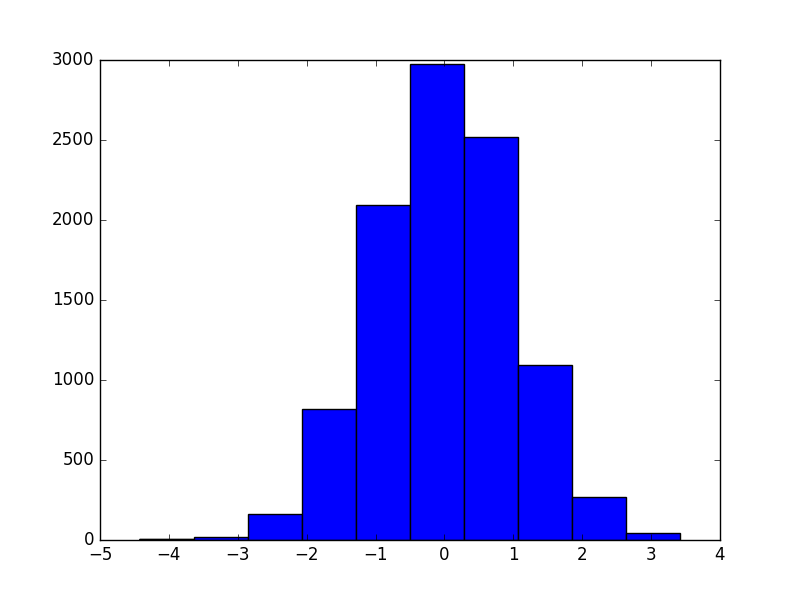
\includegraphics[width=0.4\textwidth]{./hist-normal.png}

Which of the following programs could produce this plot?  Assume that NumPy and MatPlotLib have been imported as customary in class.  Also assume that all programs work as written.
\begin{answers}
\answer
  \begin{Verbatim}
x = np.random.uniform( size=(10000,1) )
plt.plot( x )
plt.show()
  \end{Verbatim}
\correctanswer
  \begin{Verbatim}
x = np.random.randn( 10000,1 )
plt.hist( x )
plt.show()
  \end{Verbatim}
\answer
  \begin{Verbatim}
x = np.random.randint( 0,10, size=(10000,1) )
plt.hist( x )
plt.show()
  \end{Verbatim}
\answer
  \begin{Verbatim}
x = np.random.uniform( size=(10000,1) )
plt.hist( x )
plt.show()
  \end{Verbatim}
\end{answers}
 
 
\newpage
 

%%%%%%%%%%%%%%%%%%%%%%%%%%%%%%%%%%%%%%%%%%%%%
\question{1}

\variant
Which of the following Python programs best simulates the roll of one twenty-sided die in the variable \texttt{x}?  (\emph{I.e.}, any number from 1--20 inclusive is equally likely to result from the die roll or program code.)
\begin{answers}
\correctanswer
  \begin{Verbatim}
x = np.random.choice( np.arange( 1,21 ) )
  \end{Verbatim}
\answer
  \begin{Verbatim}
x = np.random.shuffle( np.arange( 1,21 ) )
  \end{Verbatim}
\answer
  \begin{Verbatim}
x = np.random.randn( np.arange( 1,21 ) )
  \end{Verbatim}
\answer
  \begin{Verbatim}
x = np.random.uniform( np.arange( 1,21 ) )
  \end{Verbatim}
\end{answers}
 
 

\end{document}
